\documentclass[a4paper,11pt]{report}
\usepackage{chuan_math_gkt}
\usetikzlibrary{angles,quotes,intersections,patterns,decorations.pathreplacing}
\chuanexamsetup

\begin{document}
\examfontsize

\examsecret{绝密$\bigstar$启用前}

\examtitle{2020年普通高等学校招生全国统一考试（全国乙卷理科）}{数\quad 学}

\noticetitle
\begin{examnotice}
\item 答卷前，考生务必将自己的姓名、准考证号填写在答题卡上. 
\item 回答选择题时，选出每小题的答案后，用铅笔把答题卡上对应题目的答案标号涂黑. 如需改动，用橡皮擦干净后，再选涂其他答案标号. 回答非选择题时，将答案写在答题卡上. 写在本试卷上无效. 
\item 考试结束后，将本试卷和答题卡一并交回. 
\end{examnotice}

\examsection{一、选择题：本题共12小题，每小题5分，共60分. 在每小题给出的四个选项中，只有一项是符合题目要求的. }
\begin{examquestions}

\item 若 $z=1+\mathrm{i}$，则 $|z^2-2z|=$
\fourchoices{$0$}{$1$}{$\sqrt{2}$}{$2$}

\item 设集合 $A=\{x\mid x^2-4\leq 0\}$，$B=\{x\mid 2x+a\leq 0\}$，且 $A\cap B=\{x\mid -2\leq x\leq 1\}$，则 $a=$
\fourchoices{$-4$}{$-2$}{$2$}{$4$}

\item 埃及胡夫金字塔是古代世界建筑奇迹之一，它的形状可视为一个正四棱锥. 以该四棱锥的高为边长的正方形面积等于该四棱锥一个侧面三角形的面积，则其侧面三角形底边上的高与底面正方形的边长的比值为

\begin{tightcenter}
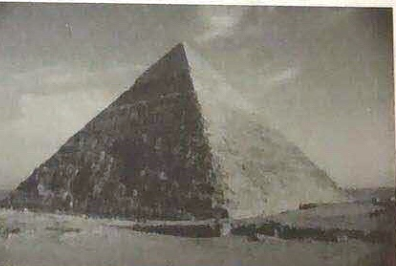
\includegraphics[width=6cm]{figures/2020_xkb1_li_image3.png}
\end{tightcenter}

\fourchoices
{\tallchoice{$\dfrac{\sqrt{5}-1}{4}$}}
{\tallchoice{$\dfrac{\sqrt{5}-1}{2}$}}
{\tallchoice{$\dfrac{\sqrt{5}+1}{4}$}}
{\tallchoice{$\dfrac{\sqrt{5}+1}{2}$}}

\item 已知点 $A$ 为抛物线 $C:y^2=2px(p>0)$ 上一点，点 $A$ 到 $C$ 的焦点的距离为 $12$，到 $y$ 轴的距离为 $9$，则 $p=$
\fourchoices{$2$}{$3$}{$6$}{$9$}

\item 某校一个课外学习小组为研究某作物种子的发芽率 $y$ 和温度 $x$（单位：$^\circ\mathrm C$）的关系，在 $20$ 个不同的温度条件下进行种子发芽实验，得到实验数据 $(x_i,y_i)(i=1,2,\ldots,20)$，得到下面的散点图：

\begin{tightcenter}
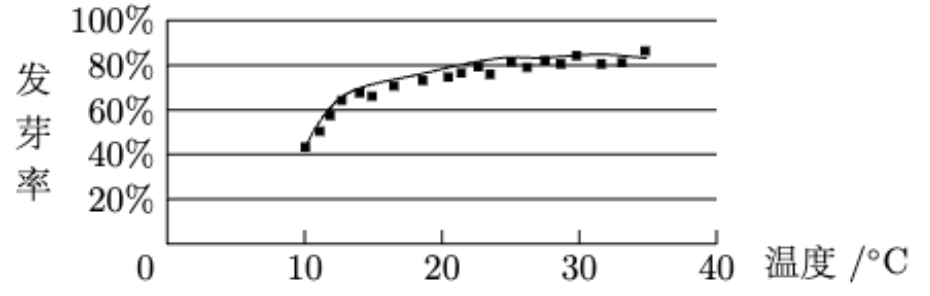
\includegraphics[width=9cm]{figures/2020_xkb1_li_image8.png}
\end{tightcenter}

由此散点图，在 $10^\circ\mathrm C$ 到 $40^\circ\mathrm C$ 之间，下面四个回归方程类型中最适宜作为发芽率 $y$ 和温度 $x$ 的回归方程类型的是
\fourchoices{$y=a+bx$}{$y=a+bx^2$}{$y=a+be^x$}{$y=a+b\ln x$}

\item 函数 $f(x)=x^4-2x^3$ 的图像在点 $(1,f(1))$ 处的切线方程为
\fourchoices{$y=-2x-1$}{$y=-2x+1$}{$y=2x-3$}{$y=2x+1$}

\item 设函数 $f(x)=\cos\left(\omega x+\dfrac{\pi}{6}\right)$ 在 $[-\pi,\pi]$ 的图像大致如下图，则 $f(x)$ 的最小正周期为

\begin{tightcenter}
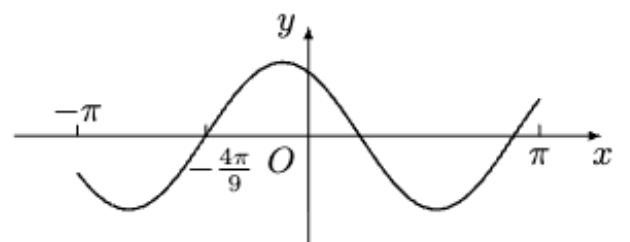
\includegraphics[width=6cm]{figures/2020_xkb1_li_image10.png}
\end{tightcenter}

\fourchoices
{\tallchoice{$\dfrac{10\pi}{9}$}}
{\tallchoice{$\dfrac{7\pi}{6}$}}
{\tallchoice{$\dfrac{4\pi}{3}$}}
{\tallchoice{$\dfrac{3\pi}{2}$}}

\item $\left(x+\dfrac{y^2}{x}\right)(x+y)^5$ 的展开式中 $x^3y^3$ 的系数为
\fourchoices{$5$}{$10$}{$15$}{$20$}

\item 已知 $\alpha\in(0,\pi)$，且 $3\cos2\alpha-8\cos\alpha=5$，则 $\sin\alpha=$
\fourchoices
{\tallchoice{$\dfrac{\sqrt5}{3}$}}
{\tallchoice{$\dfrac{2}{3}$}}
{\tallchoice{$\dfrac{1}{3}$}}
{\tallchoice{$\dfrac{\sqrt5}{9}$}}

\item 已知 $A,B,C$ 为球 $O$ 的球面上的三个点，$\odot O_1$ 为 $\triangle ABC$ 的外接圆，若 $\odot O_1$ 的面积为 $4\pi$，$AB=BC=AC=OO_1$，则球 $O$ 的表面积为
\fourchoices{$64\pi$}{$48\pi$}{$36\pi$}{$32\pi$}

\item 已知 $\odot M:x^2+y^2-2x-2y-2=0$，直线 $l:2x+y+2=0$，$P$ 为 $l$ 上的动点，过点 $P$ 作 $\odot M$ 的切线 $PA,PB$，切点为 $A,B$，当 $|PM|\cdot|AB|$ 最小时，直线 $AB$ 的方程为
\fourchoices{$2x-y-1=0$}{$2x+y-1=0$}{$2x-y+1=0$}{$2x+y+1=0$}

\item 若 $2^a+\log_2a=4^b+2\log_4b$，则
\fourchoices{$a>2b$}{$a<2b$}{$a>b^2$}{$a<b^2$}

\end{examquestions}

\examsection{二、填空题：本题共4小题，每小题5分，共20分. }
\begin{examquestions}[start=13]

\item 若 $x,y$ 满足约束条件\linsys{2x+y-2\leq0\\x-y-1\geq0\\y+1\geq0}，则 $z=x+7y$ 的最大值为 \blank.

\item $\vec a,\vec b$ 为单位向量，且 $|\vec a+\vec b|=1$，则 $|\vec a-\vec b|=$ \blank.

\noindent\begin{minipage}[t]{0.72\linewidth}
\item 已知 $F$ 为双曲线 $C:\dfrac{x^2}{a^2}-\dfrac{y^2}{b^2}=1(a>0,b>0)$ 的右焦点，$A$ 为 $C$ 的右顶点，$B$ 为 $C$ 上的点，且 $BF$ 垂直于 $x$ 轴. 若 $AB$ 的斜率为 $3$，则 $C$ 的离心率为 \blank.

\item 如图，在三棱锥 $P-ABC$ 的平面展开图中，$AC=1$，$AB=AD=\sqrt3$，$AB\perp AC$，$AB\perp AD$，$\angle CAE=30^\circ$，则 $\cos\angle FCB=$ \blank.
\end{minipage}\hfill
\begin{minipage}[t]{0.24\linewidth}\vspace{0em}\centering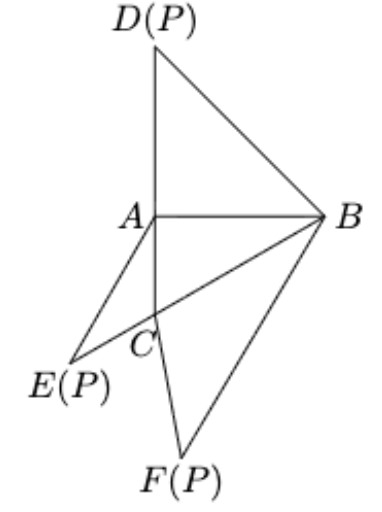
\includegraphics[width=\linewidth]{figures/2020_xkb1_li_image23.png}\end{minipage}


\end{examquestions}

\examsection{三、解答题：共70分. 解答应写出文字说明、证明过程或演算步骤. 第17题～第21题为必考题，每个试题考生都必须作答. 第22、23题为选考题，考生根据要求作答. }
\begin{examanswers}[start=17]

\item（12分）

设 $\{a_n\}$ 是公比不为 $1$ 的等比数列，$a_1$ 为 $a_2$，$a_3$ 的等差中项. 

（1）求 $\{a_n\}$ 的公比；

（2）若 $a_1=1$，求数列 $\{na_n\}$ 的前 $n$ 项和. 

\item（12分）

如图，$D$ 为圆锥的顶点，$O$ 是圆锥底面的圆心，$AE$ 为底面直径，$AE=AD$. $\triangle ABC$ 是底面的内接正三角形，$P$ 为 $DO$ 上一点，$PO=\dfrac{\sqrt6}{6}DO$. 

\begin{minipage}[t]{0.72\linewidth}
（1）证明：$PA\perp$ 平面 $PBC$；

（2）求二面角 $B-PC-E$ 的余弦值. \end{minipage}\hfill
\begin{minipage}[t]{0.26\linewidth}\vspace{-2em}\centering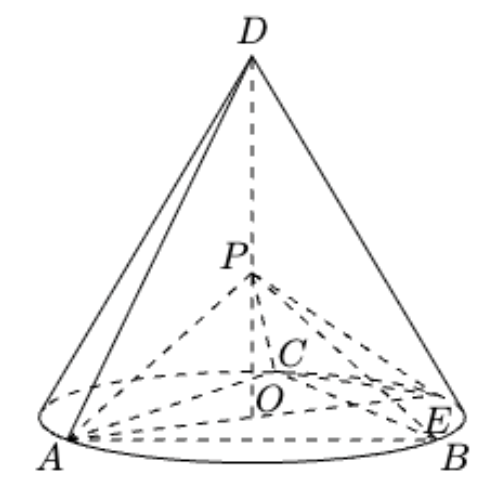
\includegraphics[width=\linewidth]{figures/2020_xkb1_li_image25.png}\end{minipage}

\vspace{-2em}
\item（12分）

甲、乙、丙三位同学进行羽毛球比赛，约定赛制如下：

累计负两场者被淘汰；比赛前抽签决定首先比赛的两人，另一人轮空；每场比赛的胜者与轮空者进行下一场比赛，负者下一场轮空，直至有一人被淘汰；当一人被淘汰后，剩余的两人继续比赛，直至其中一人被淘汰，另一人最终获胜，比赛结束. 

经抽签，甲、乙首先比赛，丙轮空. 设每场比赛双方获胜的概率都为 $\dfrac12$. 

（1）求甲连胜四场的概率；

（2）求需要进行第五场比赛的概率；

（3）求丙最终获胜的概率. 

\item（12分）

已知 $A,B$ 分别为椭圆 $E:\dfrac{x^2}{a^2}+y^2=1(a>1)$ 的左、右顶点，$G$ 为 $E$ 的上顶点，$\vec{AG}\cdot\vec{GB}=8$. $P$ 为直线 $x=6$ 上的动点，$PA$ 与 $E$ 的另一交点为 $C$，$PB$ 与 $E$ 的另一交点为 $D$. 

（1）求 $E$ 的方程；

（2）证明：直线 $CD$ 过定点. 

\item（12分）

已知函数 $f(x)=e^x+ax^2-x$. 

（1）当 $a=1$ 时，讨论 $f(x)$ 的单调性；

（2）当 $x\geq0$ 时，$f(x)\geq\dfrac12x^3+1$，求 $a$ 的取值范围. 

\item（10分）【选修4-4：坐标系与参数方程】

在直角坐标系 $xOy$ 中，曲线 $C_1$ 的参数方程为\linsys{x=\cos^k t\\y=\sin^k t}（$t$ 为参数）. 以坐标原点为极点，$x$ 轴正半轴为极轴建立极坐标系，曲线 $C_2$ 的极坐标方程为 $4\rho\cos\theta-16\rho\sin\theta+3=0$. 

（1）当 $k=1$ 时，$C_1$ 是什么曲线？

（2）当 $k=4$ 时，求 $C_1$ 与 $C_2$ 的公共点的直角坐标. 

\item（10分）【选修4-5：不等式选讲】

已知函数 $f(x)=|3x+1|-2|x-1|$. 

\begin{minipage}[t]{0.6\linewidth}
（1）画出 $y=f(x)$ 的图像；

（2）求不等式 $f(x)>f(x+1)$ 的解集. 
\end{minipage}\hfill
\begin{minipage}[t]{0.4\linewidth}\vspace{-3em}\centering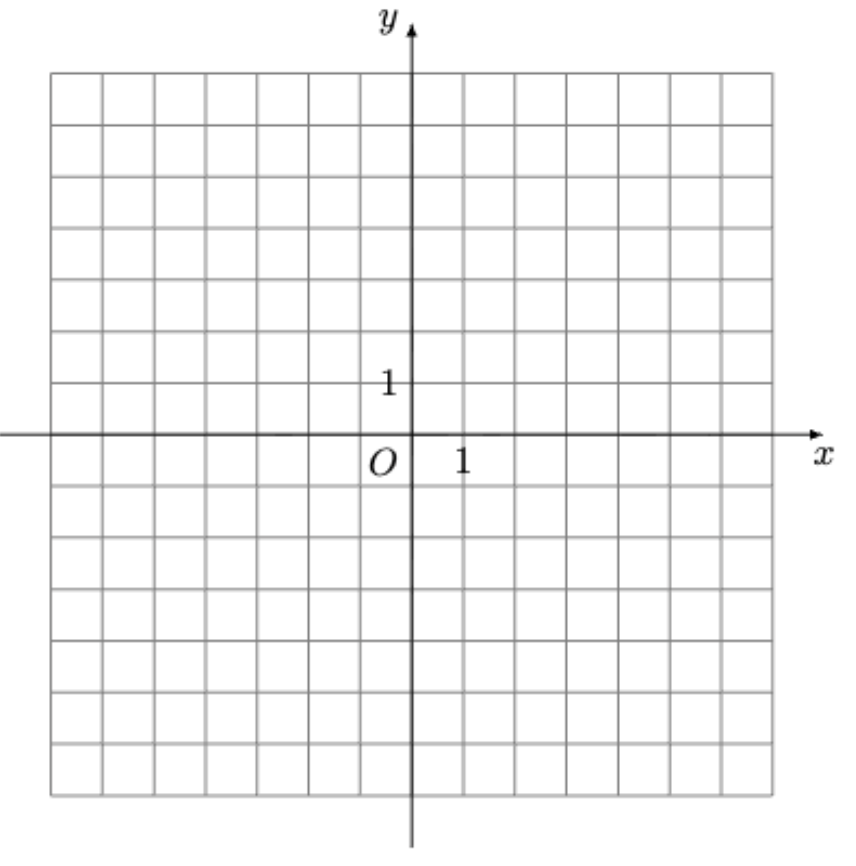
\includegraphics[width=\linewidth]{figures/2020_xkb1_li_image30.png}\end{minipage}

\end{examanswers}

\end{document}